\section{Introduction}

With our simple expressions for the reservation price and quote
spread derived from our approximations, and the intuitive procedure
described at the end of section \ref{sec:3.8}, we can easily test 
the performance of our strategy using numerical simulation. In the
first section, we will replicate the results obtained by \cite{AS2008}
and give the full python implementation.

\section{Numerical Simulations - Avellaneda \& Stoikov}

First, we need to import a couple of libraries and set up some 
auxiliary functions. The only libraries required are numpy for 
easy sampling and dealing with vectors, and matplotlib for 
producing the plots and charts later on. 

\begin{lstlisting}[language=Python, caption=Auxiliary Functions]
import numpy as np
import matplotlib as plt
        
def computeReservePrice(s,q,gamma,sigma,t,T):
    return s-q*gamma*(sigma**2)*(T-t)

def computeSpread(gamma,sigma,t,T,k):
    return (gamma * (sigma ** 2) * (T-t)) + ((2 / gamma) * 
        np.log(1 + (gamma / k)))

def computeRate(A,k,delta):
    return A*np.exp(-k*delta)

def computeSamplePath(S0, sigma, dt, T):
    return np.insert(S0 + np.cumsum(sigma * np.sqrt(dt) * 
        np.random.choice([1,-1], int(T/dt))), 0, S0)
\end{lstlisting}

\texttt{computeReservePrice} takes the current stock price, current
inventory, risk aversion, volatility, current time and end time as
arguments and returns the current reservation price as given in 
(\ref{eq:3.34}).

\texttt{computeSpread} takes the risk aversion, volatility, current
time, end time and orderbook parameter $k$ as arguments and computes
the current spread as given by (\ref{eq:3.35}).

\texttt{computeRate} computes the function $\lambda$ in the form assumed
by (\ref{eq:3.24}), taking the orderbook parameters $A$ and $k$ and the 
current spread $\delta$ as arguments.

\texttt{computeSamplePath} generates a sample path from a brownian motion
from $t$ to $T$ with stepsize $\mathrm dt$, volatility $\sigma$ and starting
value $S_0$.

Next, we define a function which we can call as many times as we 
would like to compare the performance of our ``inventory'' strategy
derived in chapter \ref{chap:3} to that of a benchmark ``symmetric''
strategy, where we compute the average spread over time of the inventory
strategy and constantly maintain this spread symmetric about the midprice,
regardless of our inventory. Comments are included throughout the code.
We use the same parameters as \cite{AS2008}, namely $S_0=100$,
$T=1$, $\sigma=2$, $\mathrm dt=0.005$, $k=1.5$, $A=140$, and $q_0=0$.

\begin{lstlisting}[language=Python, caption=Avellaneda-Stoikov Model]
def simulateBothStrategies(gamma, plots=False):
    # Initialise model parameters
    S0 = 100
    T = 1
    sigma = 2
    dt = 0.005
    k = 1.5
    A = 140

    # Initialise variables to keep track of inventory strategy
    inv_q = 0
    inv_X = 0
    inv_bids = []
    inv_asks = []
    inv_wealth = []
    inv_adj_wealth = []
    inv_inventory = []

    # Initialise variables to keep track of symmetric strategy
    sym_q = 0 
    sym_X = 0
    sym_bids=[]
    sym_asks=[]
    sym_wealth = []
    sym_adj_wealth = []
    sym_inventory = []

    # generate sample path for midprice
    price_process = computeSamplePath(S0, sigma, dt, T)

    # compute average inventory strat spread over sample path
    sym_spread = 0 
    for i in np.arange(0, T, dt):
        sym_spread += computeSpread(gamma, sigma, i, T, k)
        av_sym_spread = (sym_spread / (T / dt))
        sym_prob = min(A*np.exp(-k*av_sym_spread / 2) * dt, 1)
        sym_bids = price_process - av_sym_spread/2
        sym_asks = price_process + av_sym_spread/2

    # iterate through price process
    for step, s in enumerate(price_process):
        # compute reserve price and spread
        r = computeReservePrice(s,inv_q,gamma,sigma,step*dt,T)
        spread = computeSpread(gamma, sigma, step*dt, T, k) / 2
        delta_a = (spread + r) - s
        delta_b = s - (r - spread)

        # keep track of any updated variables
        inv_asks.append(s + delta_a)
        inv_bids.append(s - delta_b)
        inv_wealth.append(inv_X)
        inv_adj_wealth.append(inv_X + inv_q * s)
        inv_inventory.append(inv_q)

        # sample possible incoming market orders
        prob_a = min(computeRate(A,k,delta_a) * dt, 1)
        prob_b = min(computeRate(A,k,delta_b) * dt, 1)
        p = np.random.default_rng().uniform(0,1,None)
        if p <= prob_a:
            inv_q -= 1
            inv_X += (s+delta_a)
        p = np.random.default_rng().uniform(0,1,None)
        if p <= prob_b:
            inv_q += 1
            inv_X -= (s-delta_b)

        # keep track of symmetric strategy
        sym_wealth.append(sym_X) 
        sym_adj_wealth.append(sym_X + sym_q * s)
        sym_inventory.append(sym_q)

        # sample incoming market orders for symmetric strat
        p = np.random.default_rng().uniform(0,1,None)
        if p <= sym_prob:
            sym_q -= 1
            sym_X += (s + av_sym_spread / 2)
        p = np.random.default_rng().uniform(0,1,None)
        if p <= sym_prob:
            sym_q += 1
            sym_X -= (s-av_sym_spread/2)
    
    if plots==True:
        t = np.arange(0, T+dt, dt)
        plt.plot(t, price_process, 'black', linewidth = 1.0, 
            label = "S")
        plt.plot(t, asks, 'green', linewidth=1.0,label="p_a")
        plt.plot(t, bids, 'red',linewidth=1.0,label="p_b")
        ax = plt.gca()
        ax.set_facecolor((0.9,0.9,0.9,1))
        plt.xlabel("t")
        plt.ylabel("S")
        plt.legend()
        plt.show()

        plt.plot(t, inventory, 'purple', linewidth = 1.0, 
            label = "q")
        ax = plt.gca()
        ax.set_facecolor((0.9,0.9,0.9,1))
        plt.xlabel("t")
        plt.ylabel("q")
        plt.legend()
        plt.show()

        plt.plot(t, wealth, "red", linewidth=1.0,label="X")
        plt.plot(t, adj_wealth, "blue", linewidth = 1.0, 
            label = "X+q*S")
        ax = plt.gca()
        ax.set_facecolor((0.9,0.9,0.9,1))
        plt.xlabel("t")
        plt.ylabel("X")
        plt.legend()
        plt.show()
    
    # Return final performance of both strategies
    return((inv_wealth[-1], inv_inventory[-1], 
        price_process[-1], sym_wealth[-1], 
        sym_inventory[-1], av_sym_spread))
\end{lstlisting}

Using the function above, we run 10000 simulations of both the inventory
and symmetric strategies and report means and standard deviations of 
profit ($X_T+q_TS_T$) and final inventory $q_T$. We also report the 
mean spread for the inventory strategy, which is also the spread employed
by the symmetric strategy throughout. We are also interested
in the effect of varying the risk-aversion parameter $\gamma$ on the 
final inventory and shape of the Profit and Loss (PnL) profile.

\begin{lstlisting}[language=Python, caption=run-simulations]
series = []
for i in range(10000):
    series.append(simulateBothStrategies(0.1))

series = np.array(series)
inv_final_inv = series[:,1]
inv_adj_wealth = series[:,0]+inv_final_inv*series[:,2]
print("Inventory strat mean PNL: {}".format(
    np.mean(inv_adj_wealth)))
print("Inventory strat PNL stdev: {}".format(
    np.std(inv_adj_wealth)))
print("Inventory strat final q mean: {}".format(
    np.mean(inv_final_inv)))
print("Inventory strat final q stdev: {}".format(
    np.std(inv_final_inv)))

sym_final_inv = series[:,4]
sym_adj_wealth = series[:,3]+sym_final_inv*series[:,2]
print("Symmetric strat mean PNL: {}".format(
    np.mean(sym_adj_wealth)))
print("Symmetric strat PNL stdev: {}".format(
    np.std(sym_adj_wealth)))
print("Symmetric strat final q mean: {}".format(
    np.mean(sym_final_inv)))
print("Symmetric strat final q stdev: {}".format(
    np.std(sym_final_inv)))

print("Average spread: {}".format(np.mean(series[:,5])))

bins=np.histogram(np.hstack((inv_adj_wealth,sym_adj_wealth)), 
    bins=100)[1] 
plt.hist(inv_adj_wealth, bins, alpha = 1, 
    label = "Inventory strategy", edgecolor = "white", 
    color = "red")
plt.hist(sym_adj_wealth, bins, label = "Symmetric strategy", 
    edgecolor = "black", color = "white", fc = (1,0,1,0))
plt.legend()
plt.ylim((0,1200))
plt.xlabel("PnL")
plt.ylabel("# of runs")
ax = plt.gca()
ax.set_facecolor((0.9,0.9,0.9,1))
plt.show()
\end{lstlisting}

In figure \ref{fig:results-gamma01} we have the results and PnL 
distributions for 10000 simulations with $\gamma=0.1$. We obtain 
an identical mean spread to \cite{AS2008}, which is to be expected
as the calculation for the mean spread does not depend on either 
the sampling of the mid-price nor the sampling of market orders.
All of our results for the mean and standard deviation of the profit
and final inventory are within $0.1$ of those presented in the original
paper, with the exception of the standard deviation of final inventory 
where my figure of 13.1 is 0.4 above the 12.7 reported by Avellaneda
and Stoikov.

\begin{figure}[ht!]
    \centering
        \begin{tabular}{ c c c c c c } 
            \hline
            Strategy & $\mu$ (Spread) & $\mu$ (Profit) & $\sigma$ (Profit) & $\mu$ (Final q) & $\sigma$ (Final q) \\  
            \hline
            Inventory & 1.49 & 64.9 & 6.7 & 0.03 & 2.9 \\
            Symmetric & 1.49 & 68.2 & 13.1 & -0.1 & 8.3 \\
            \hline
        \end{tabular}
        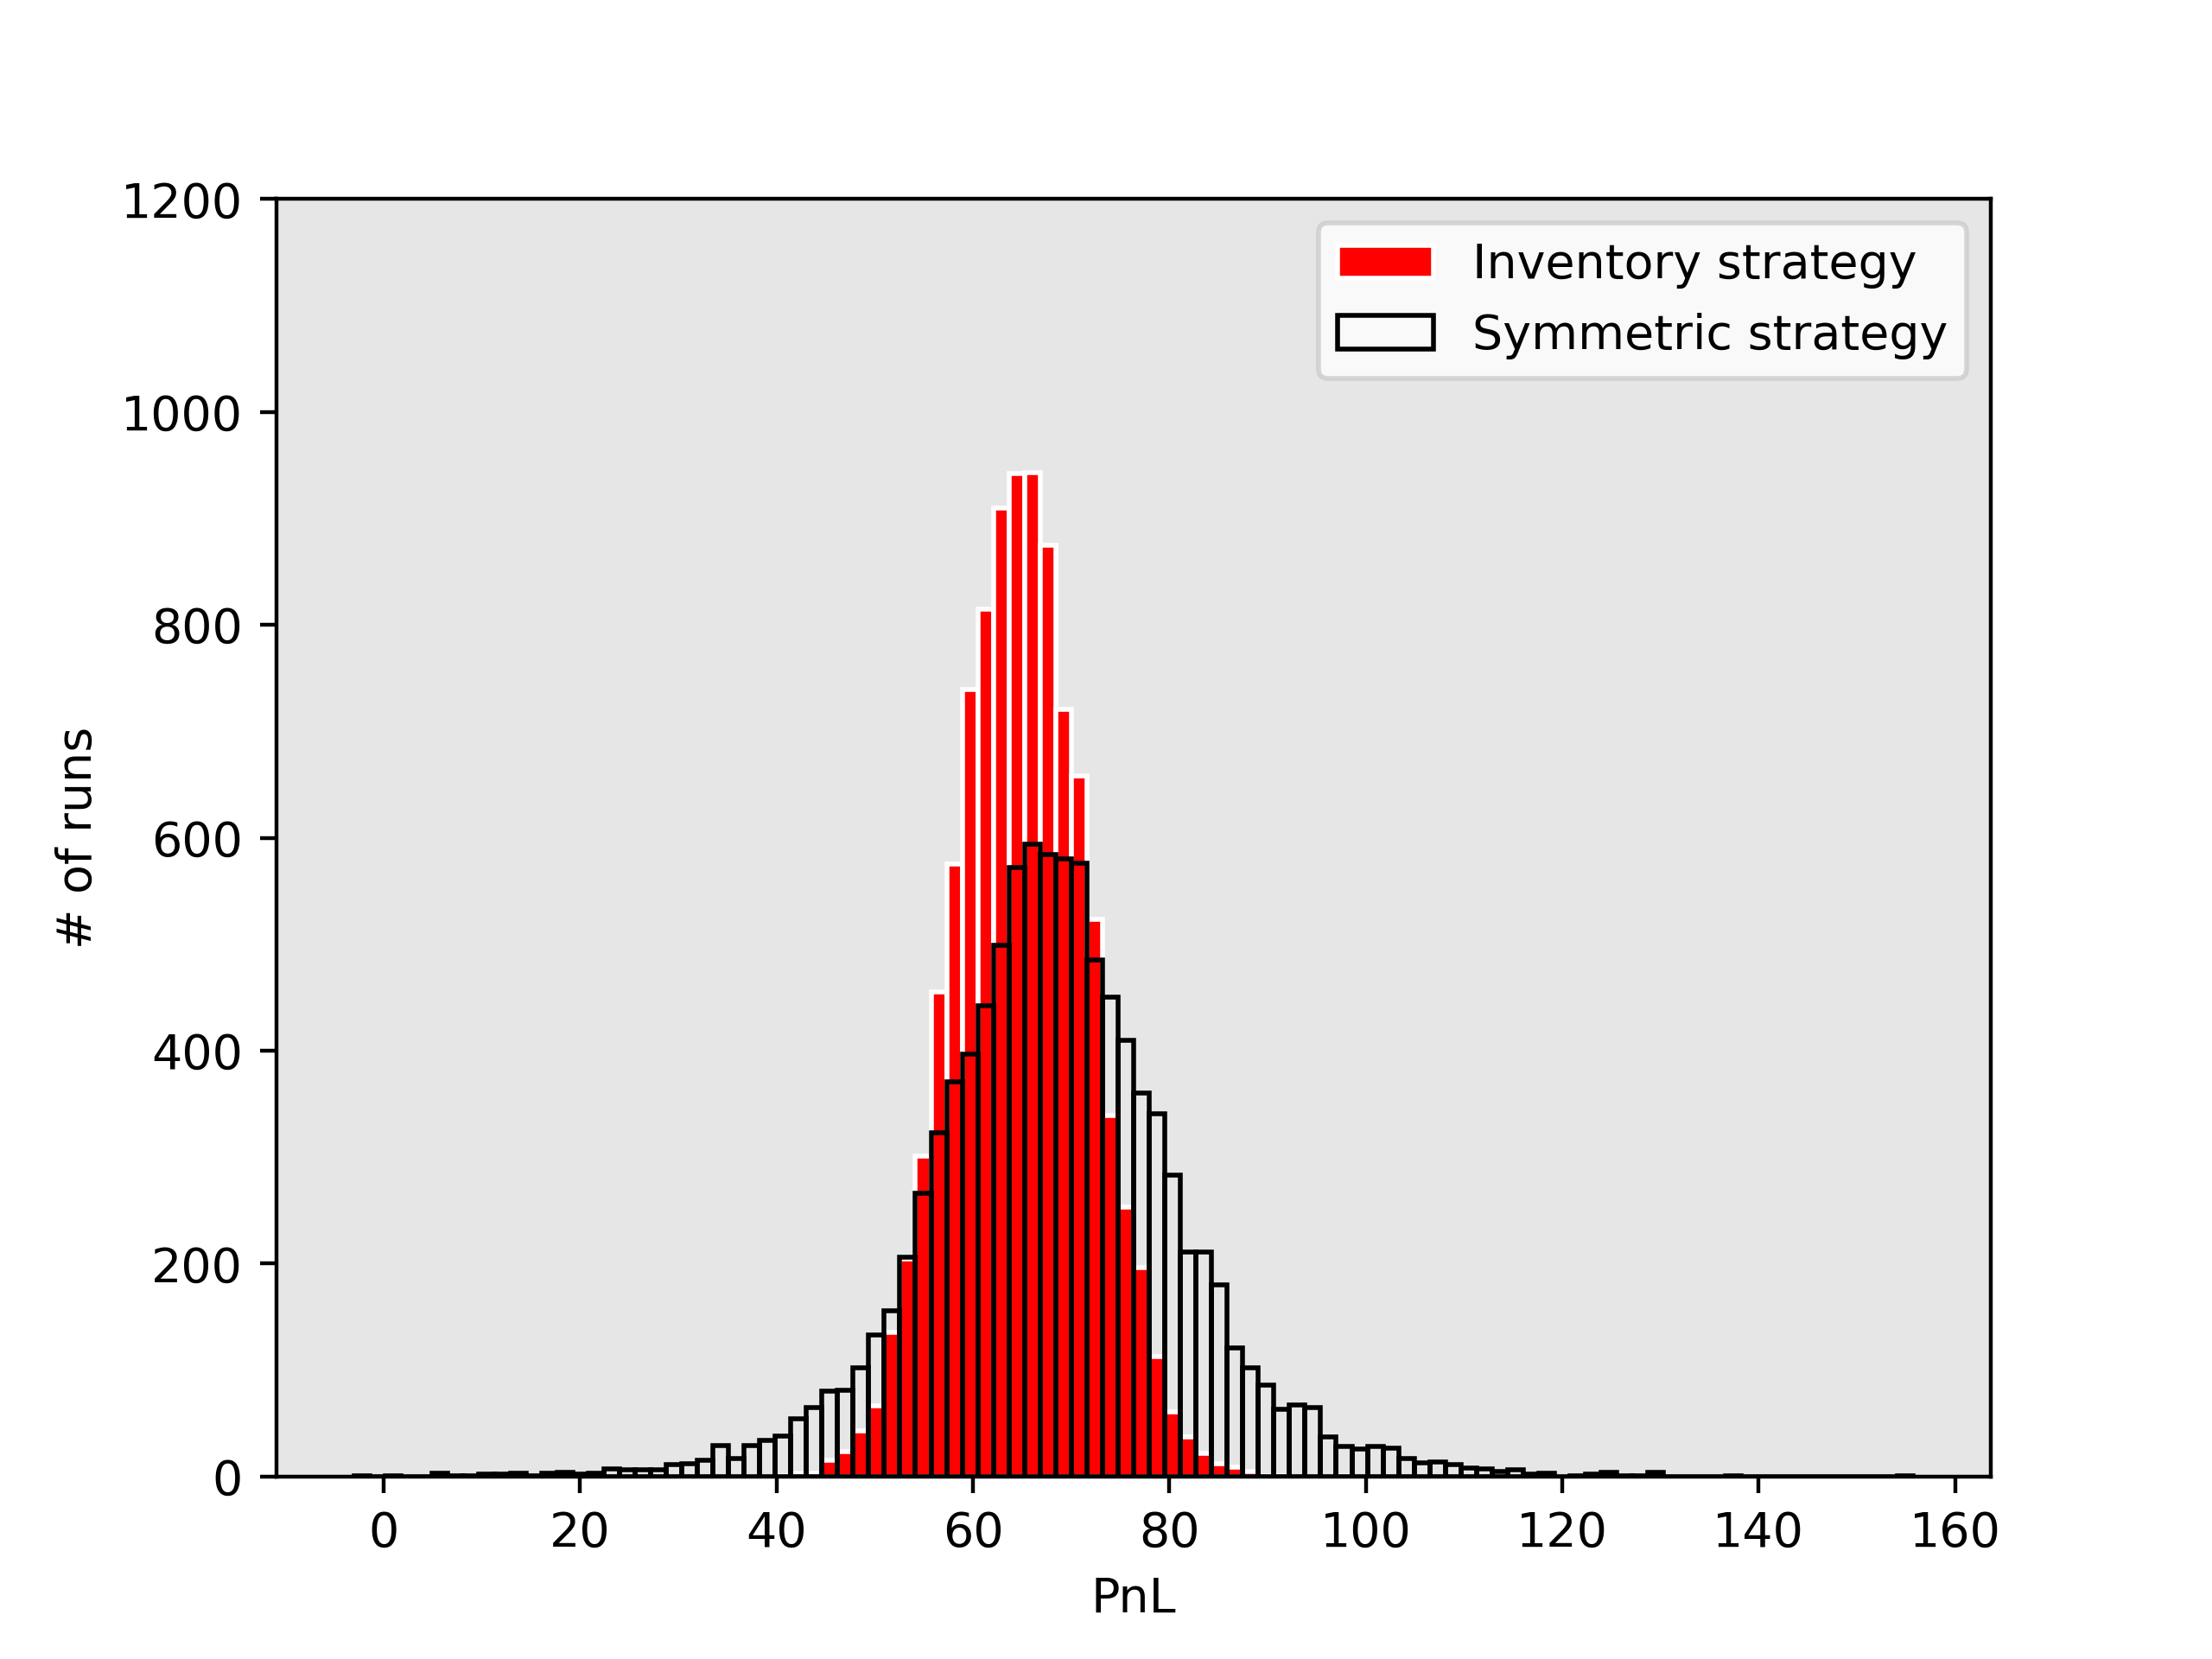
\includegraphics[scale=0.5]{gamma01.png}
        \caption{Results for $\gamma=0.1$}
        \label{fig:results-gamma01}
\end{figure}

In figure \ref{fig:results-gamma001} we present the results for 
10000 simulations with $\gamma=0.01$. Again, all of our figures 
closely match those presented by Avellaneda and Stoikov. In their 
paper, they run 1000 simulations for each level of $\gamma$, whereas
here we run 10000. Moreover, the reported results are statistical 
properties and hence it is very unlikely that we should obtain exactly
the same figures.

\begin{figure}
    \centering
        \begin{tabular}{ c c c c c c } 
            \hline
            Strategy & $\mu$ (Spread) & $\mu$ (Profit) & $\sigma$ (Profit) & $\mu$ (Final q) & $\sigma$ (Final q) \\ 
            \hline
            Inventory & 1.35 & 68.5 & 9.1 & 0.04 & 5.3 \\
            Symmetric & 1.35 & 68.6 & 13.8 & 0.04 & 8.6 \\
            \hline
        \end{tabular}
        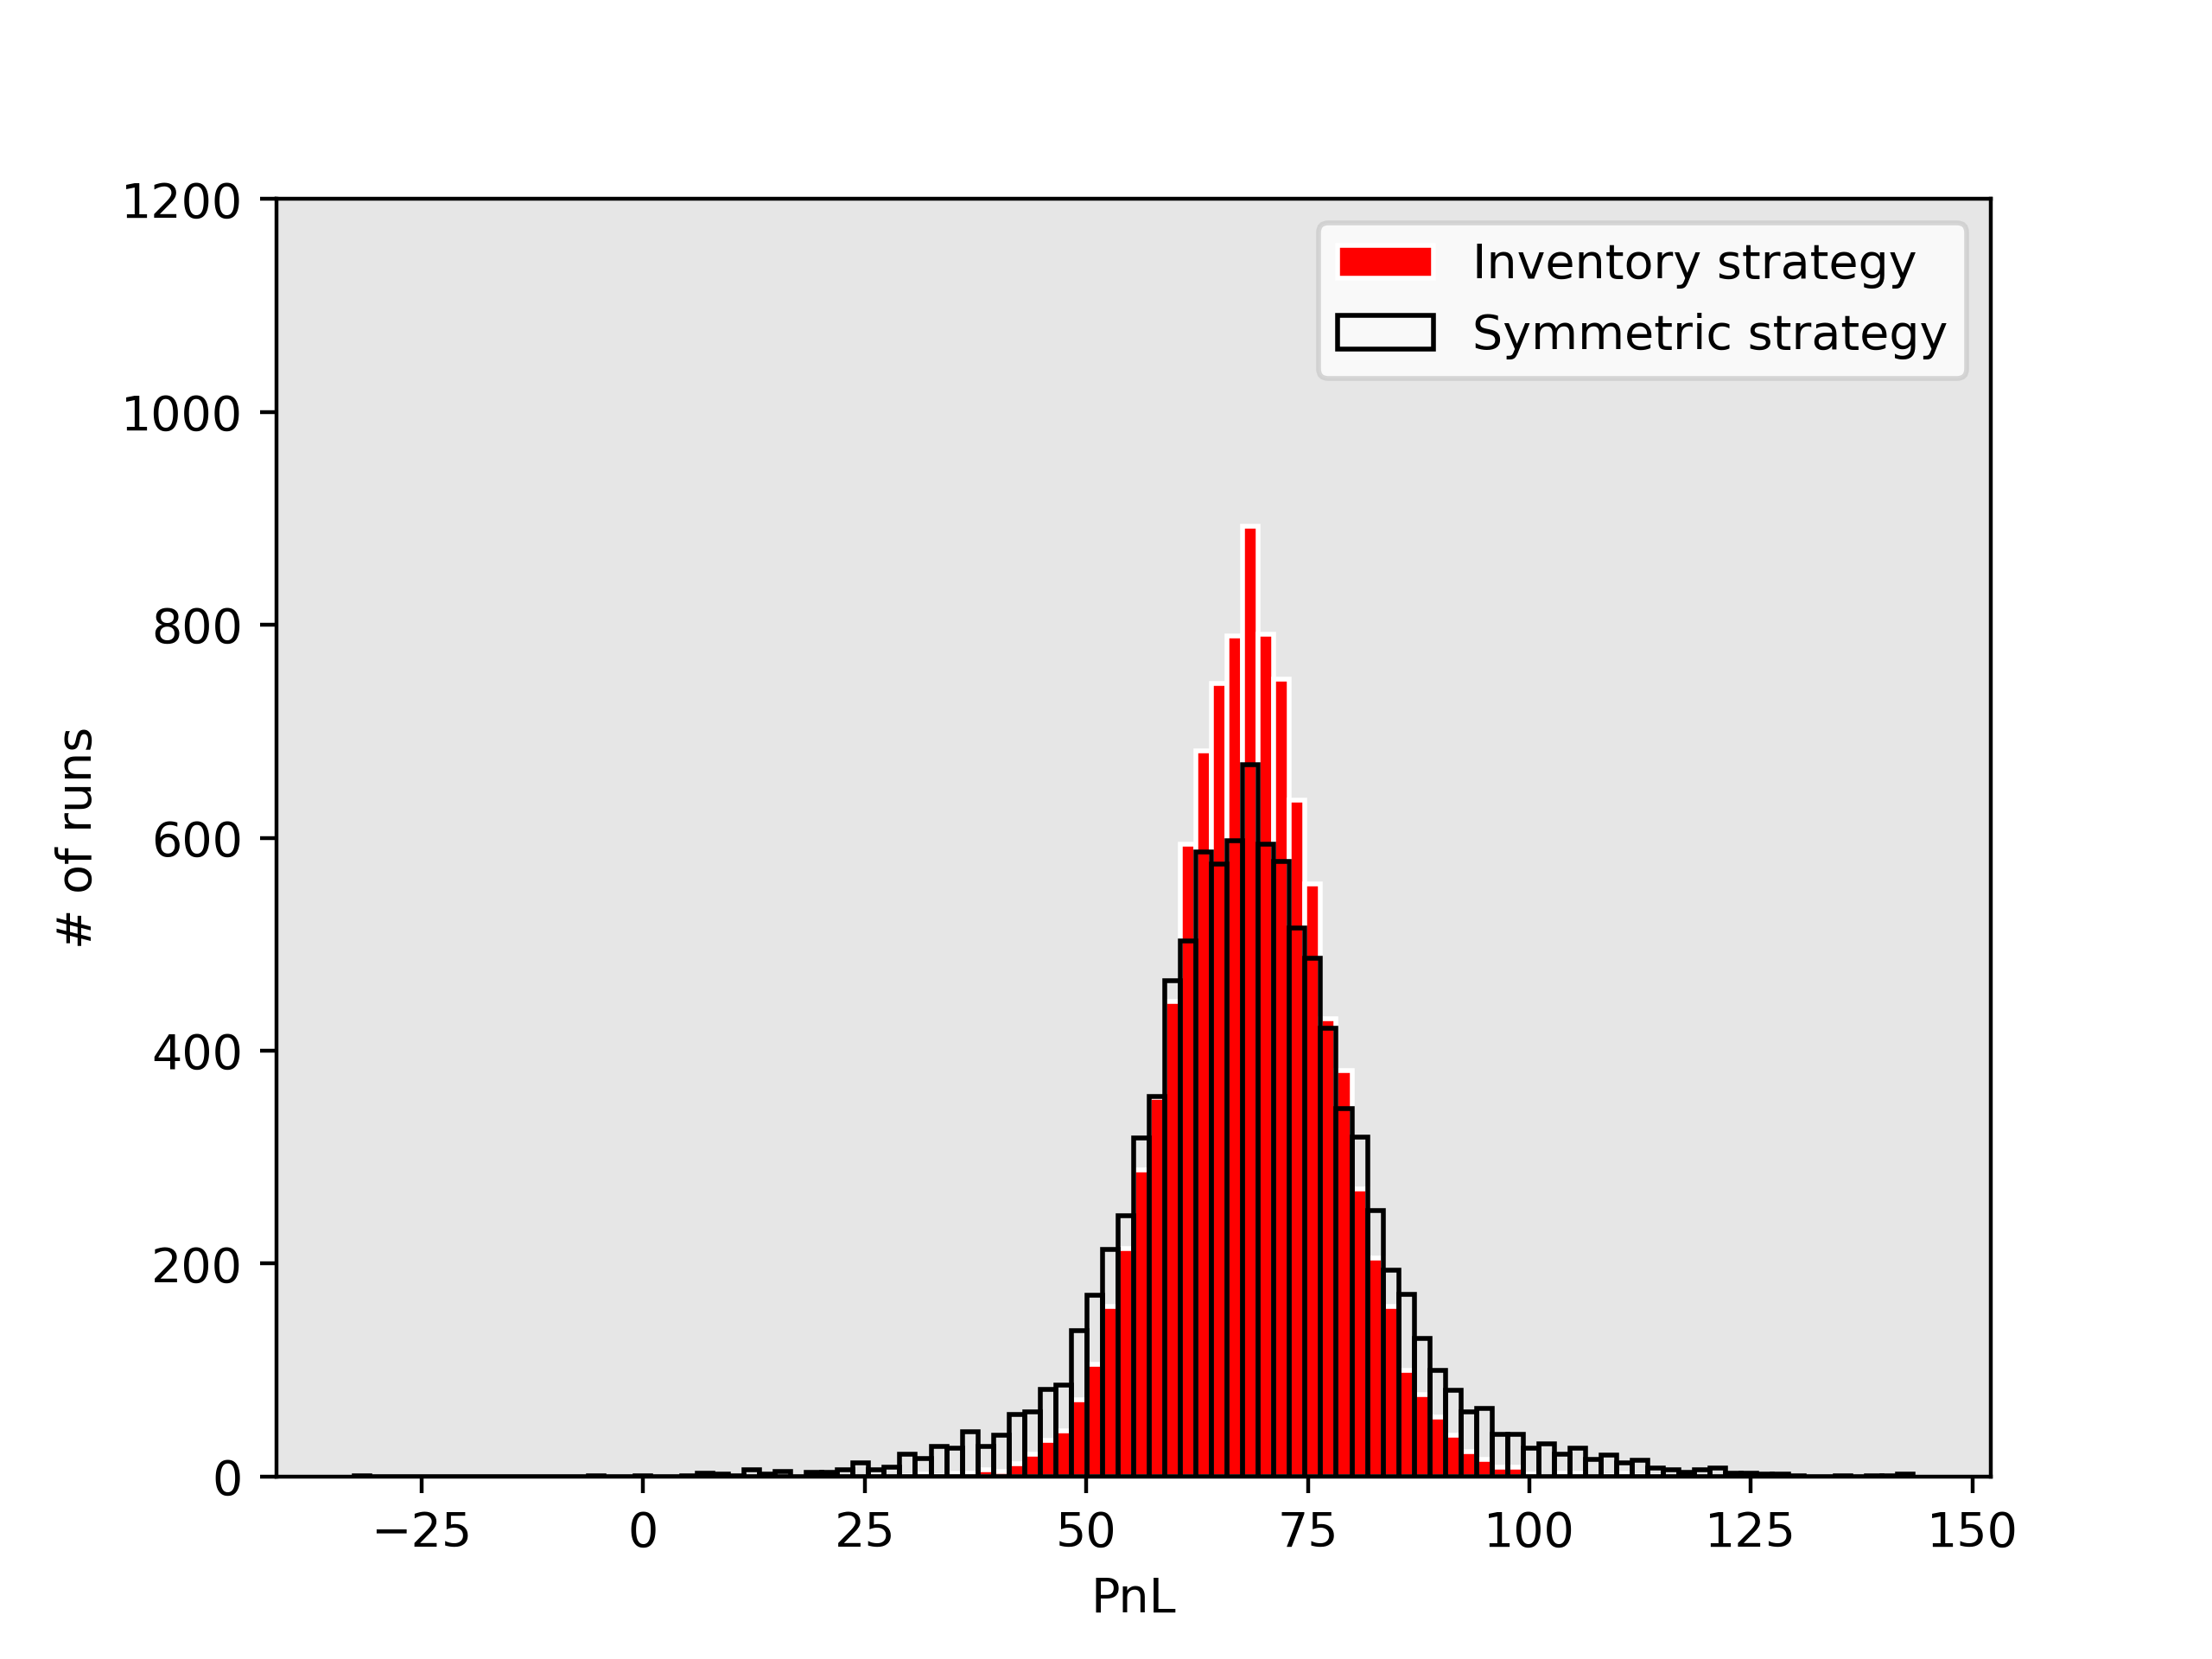
\includegraphics[scale=0.5]{gamma001.png}
        \caption{Results for $\gamma=0.01$}
        \label{fig:results-gamma001}
\end{figure}

Finally, we plot an example simulation of the model, including the 
midprice, bid and ask prices, cash flow, wealth and inventory. We 
can identify the effect of varying levels of inventory on our bid 
and ask quotes: at $t\approx0.3$ for example, the agent was short 
stock and hence set her quotes around a high reservation price, resulting
in a bid price that almost coincided with the midprice. We can also 
see the effect of time - as we reach $T$, the quotes become more 
and more symmetric as we become more and more certain about the 
terminal price $S_T$.

\begin{figure}
    \centering
        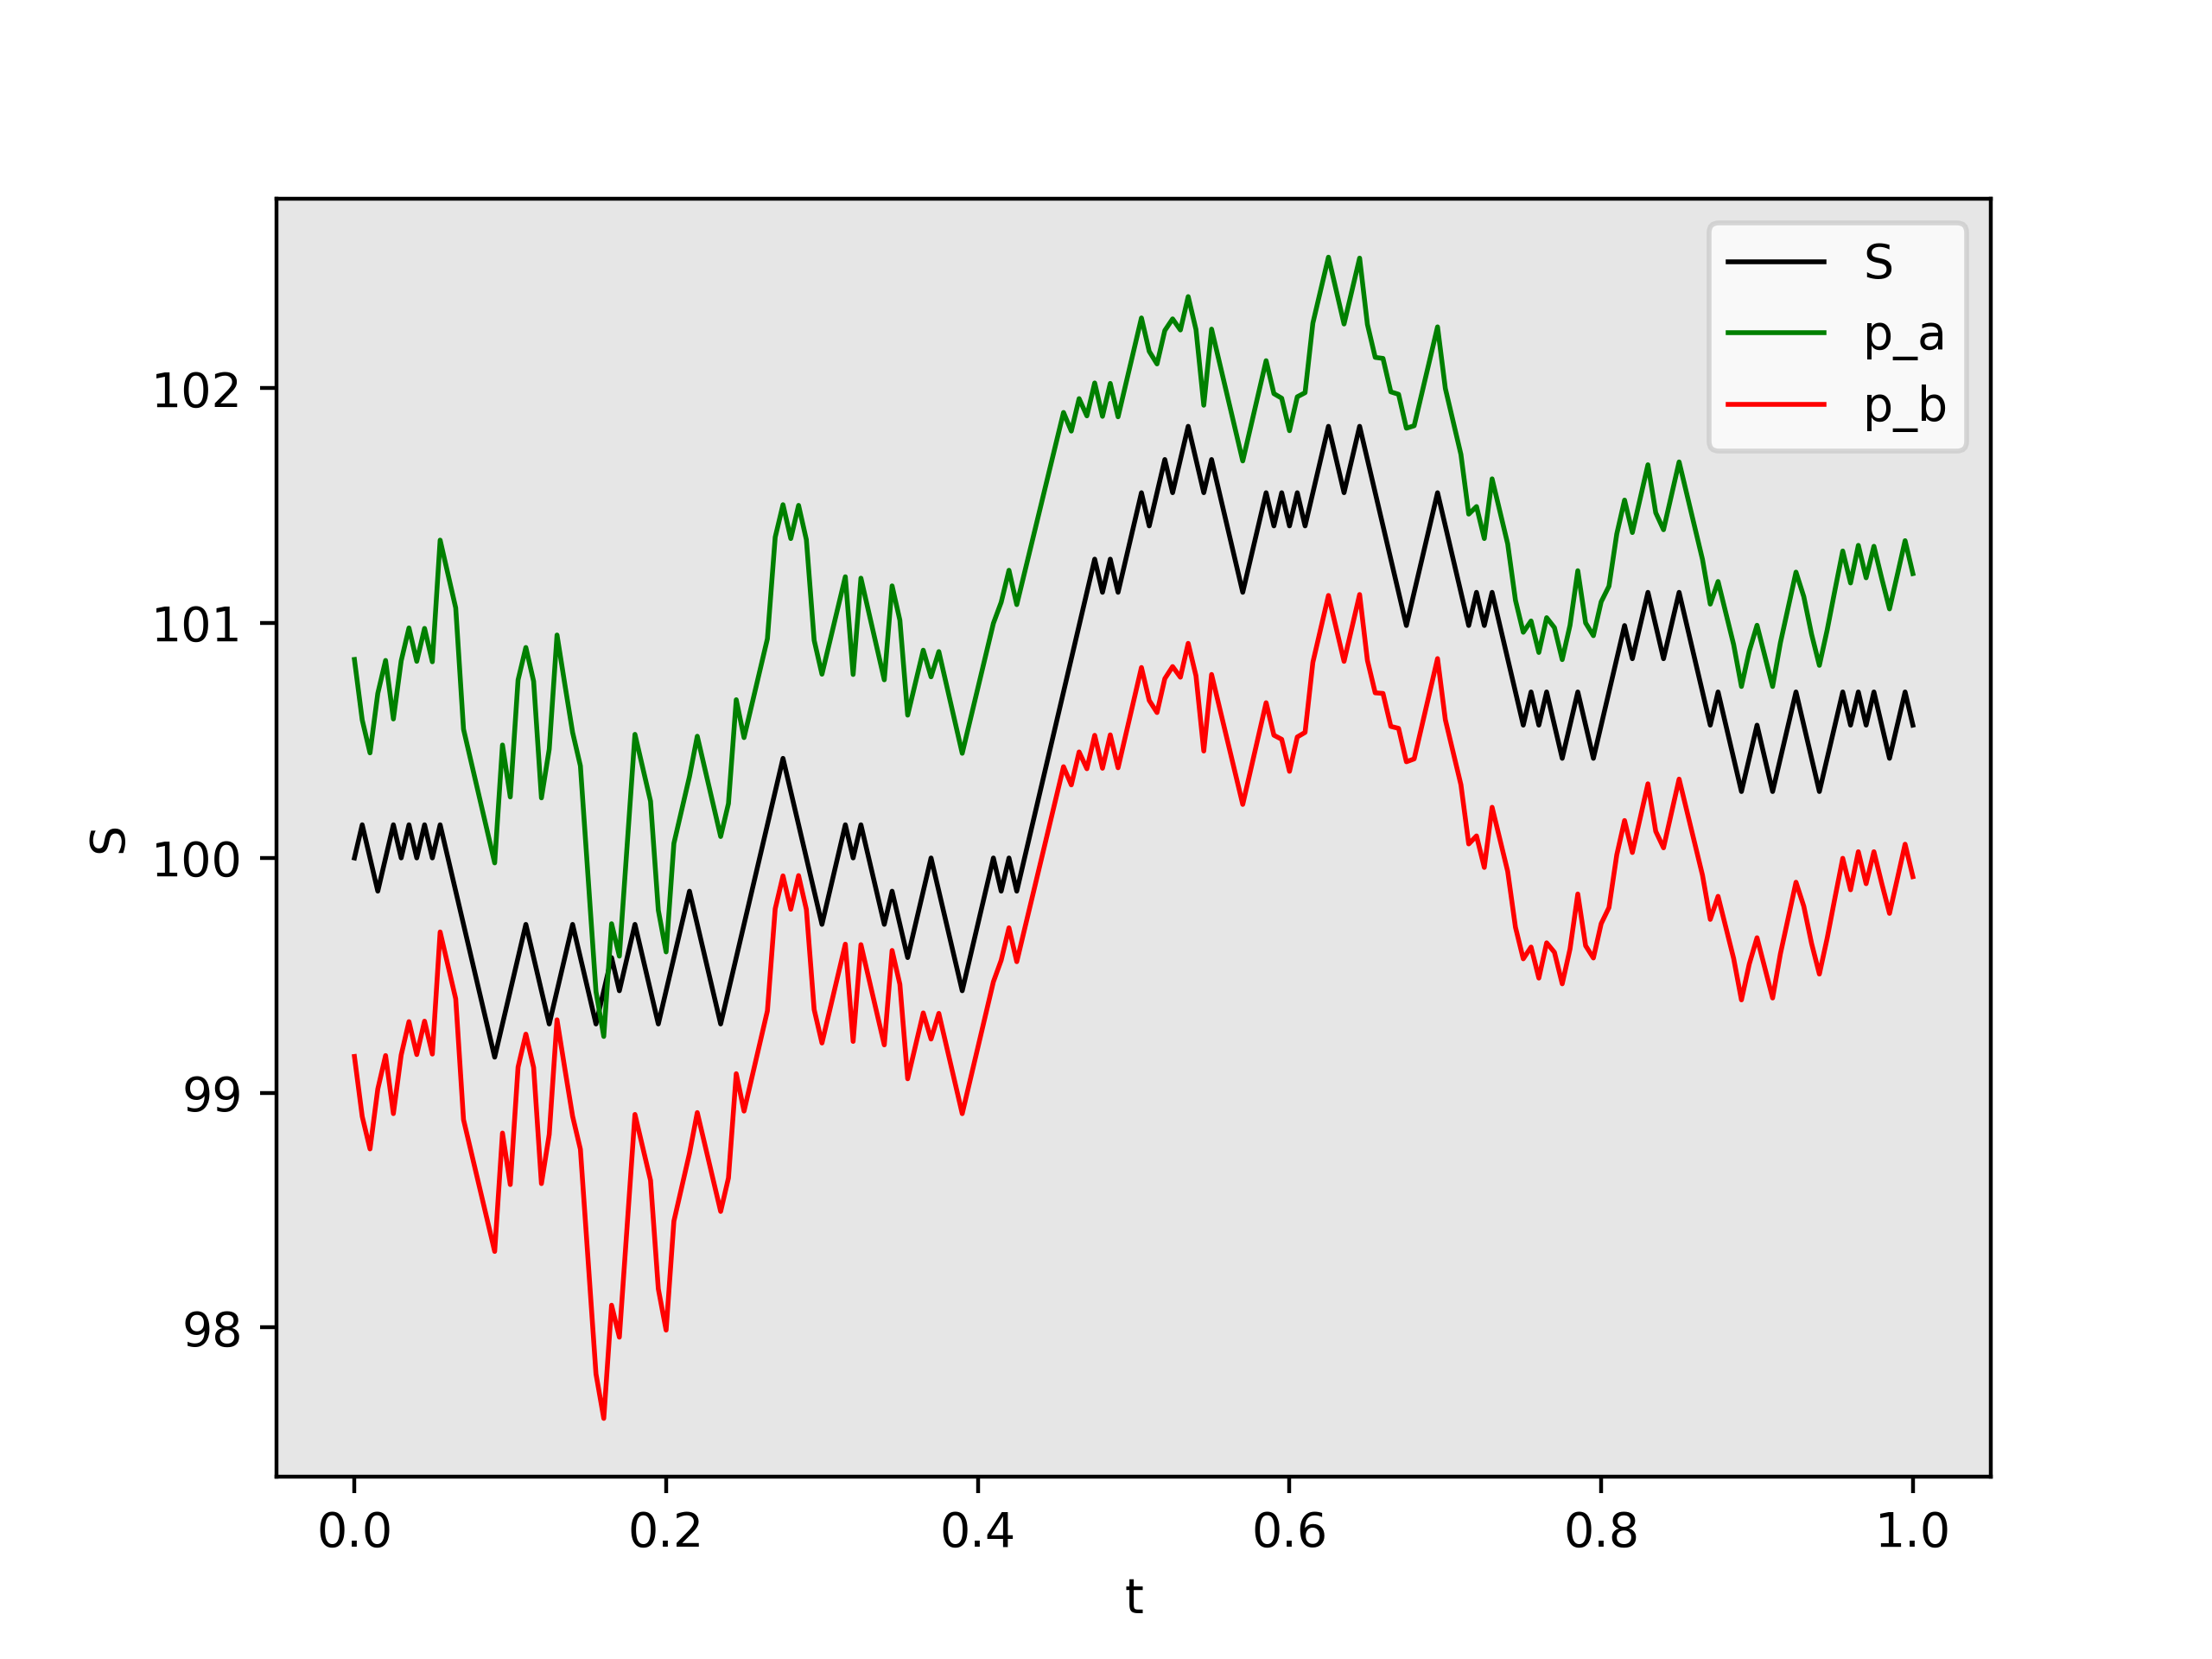
\includegraphics[scale=0.5]{sample-path.png}
        \caption{Sample path for $\gamma=0.1$}
        \label{fig:sample-paths}
\end{figure}

\begin{figure}
    \centering
        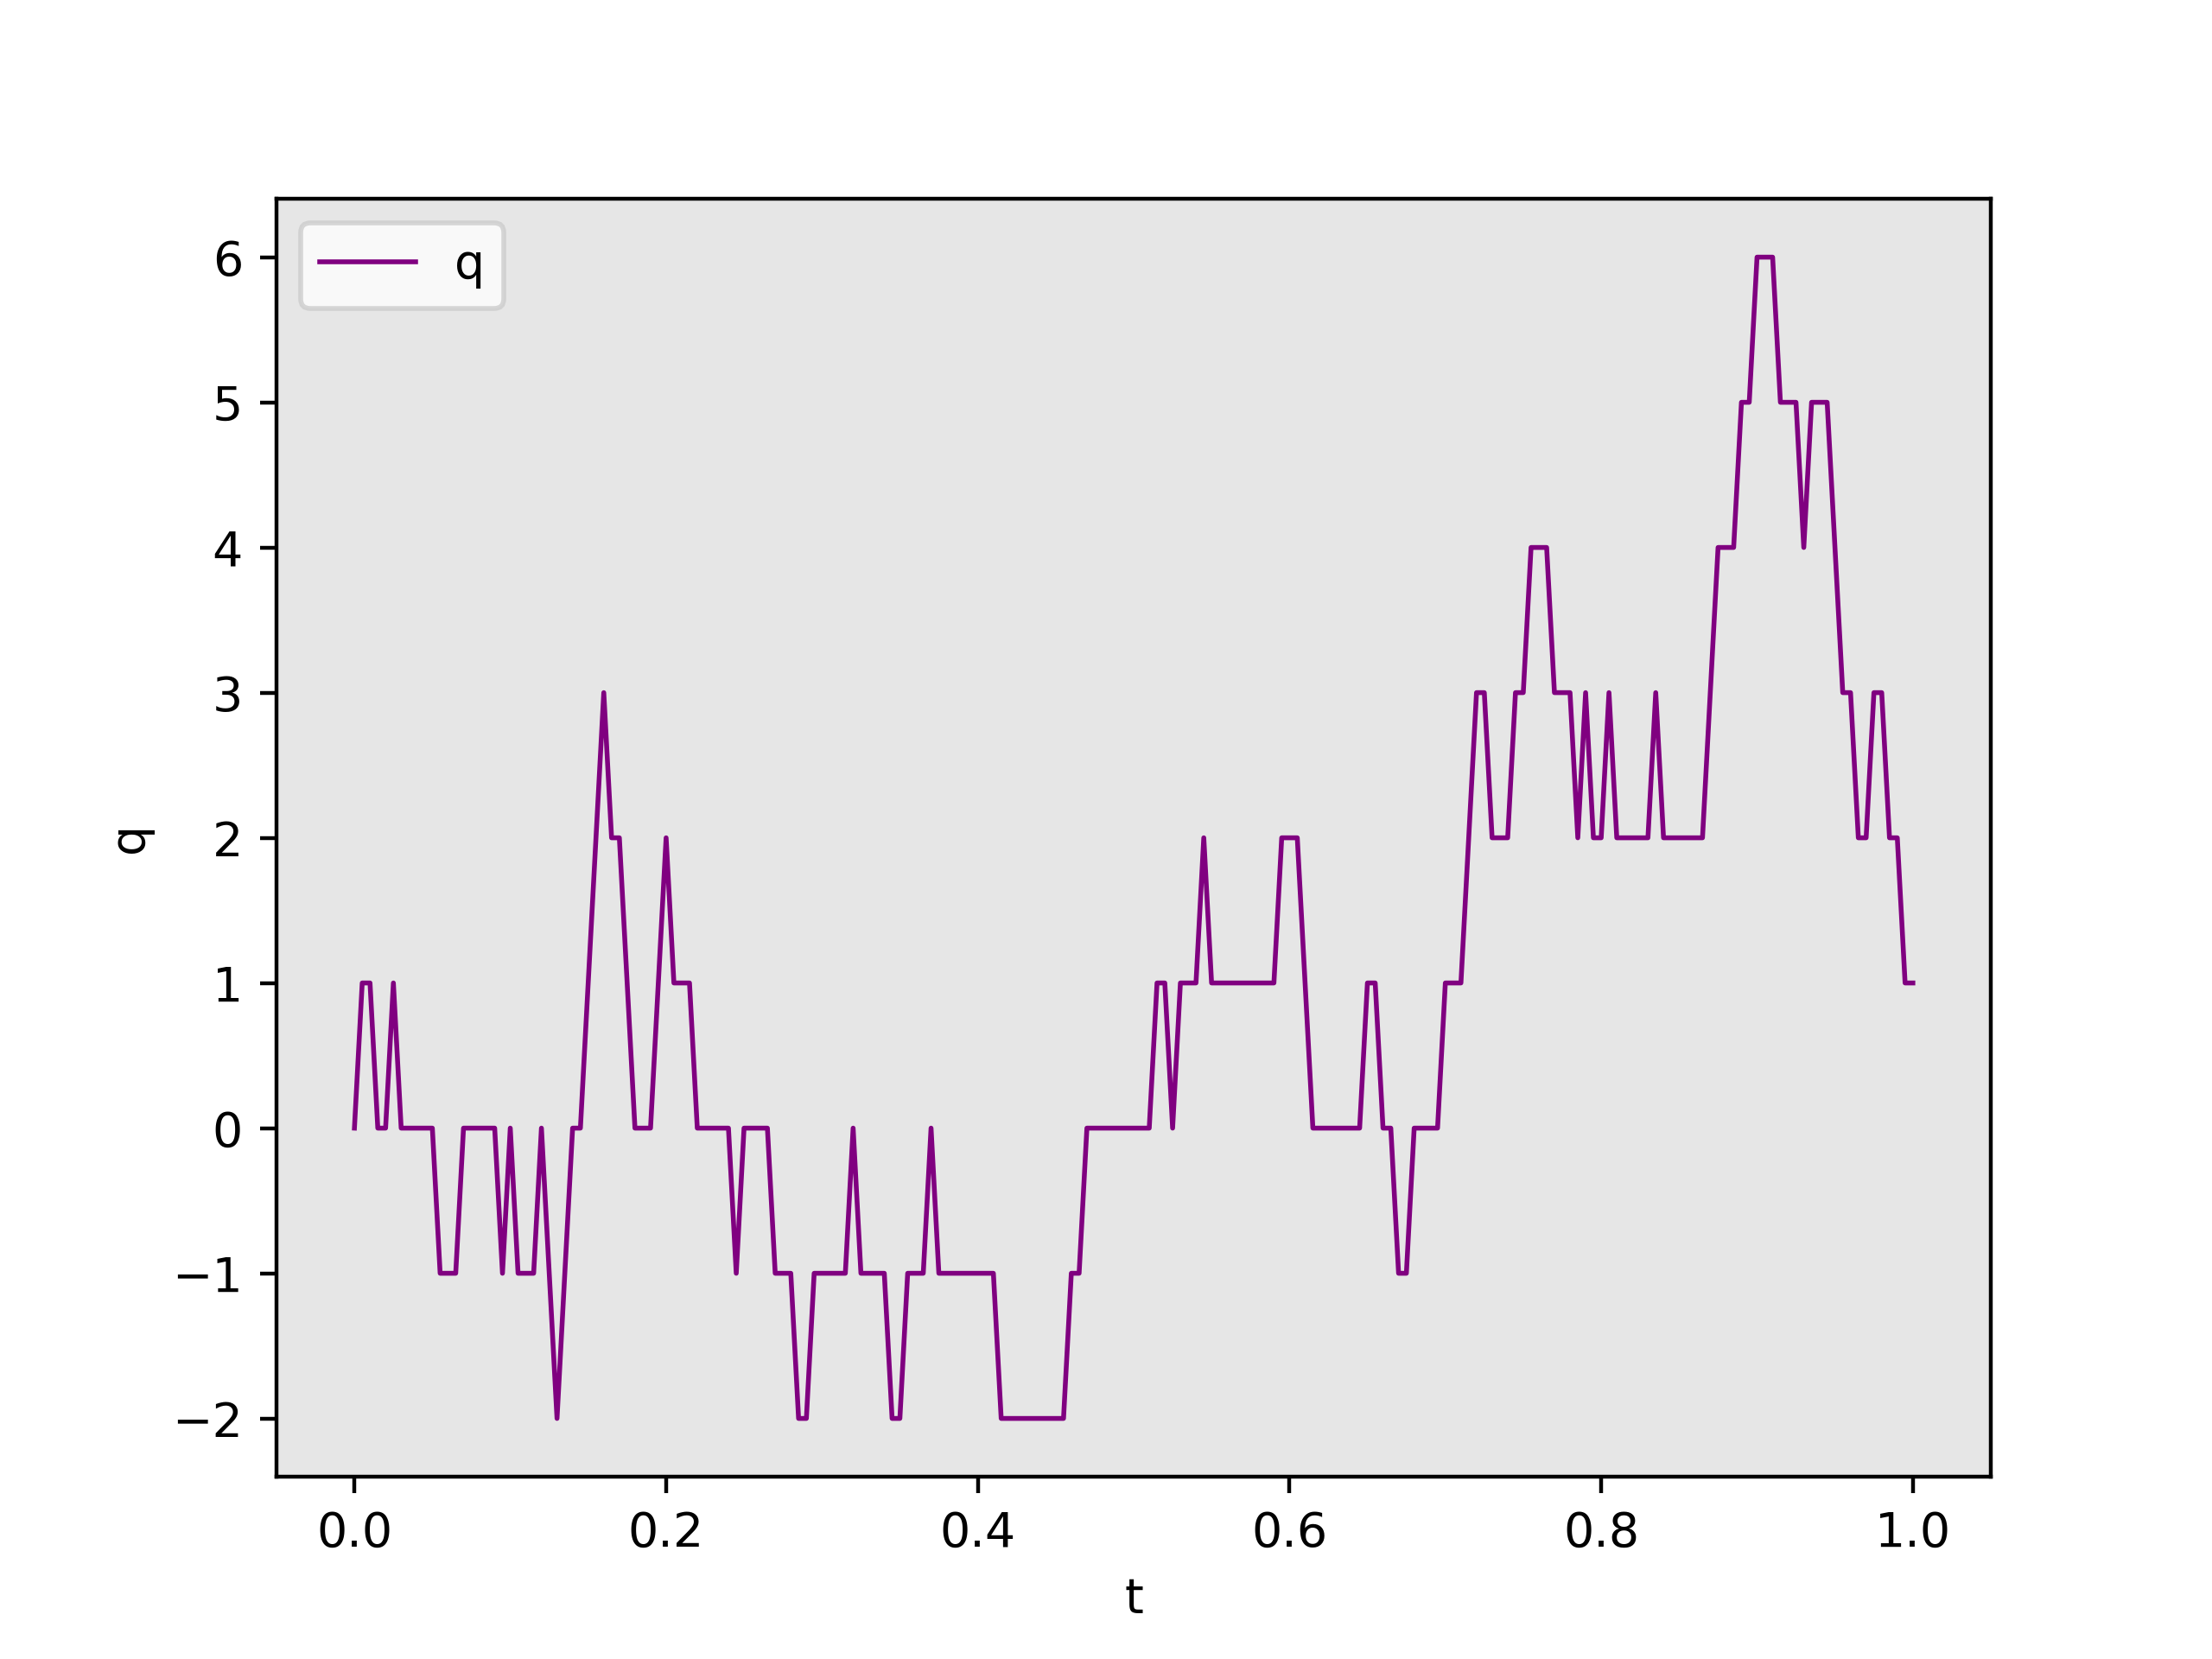
\includegraphics[scale=0.5]{inventory.png}
        \caption{Sample inventory for $\gamma=0.1$}
        \label{fig:inventory}
\end{figure}

\begin{figure}
    \centering
        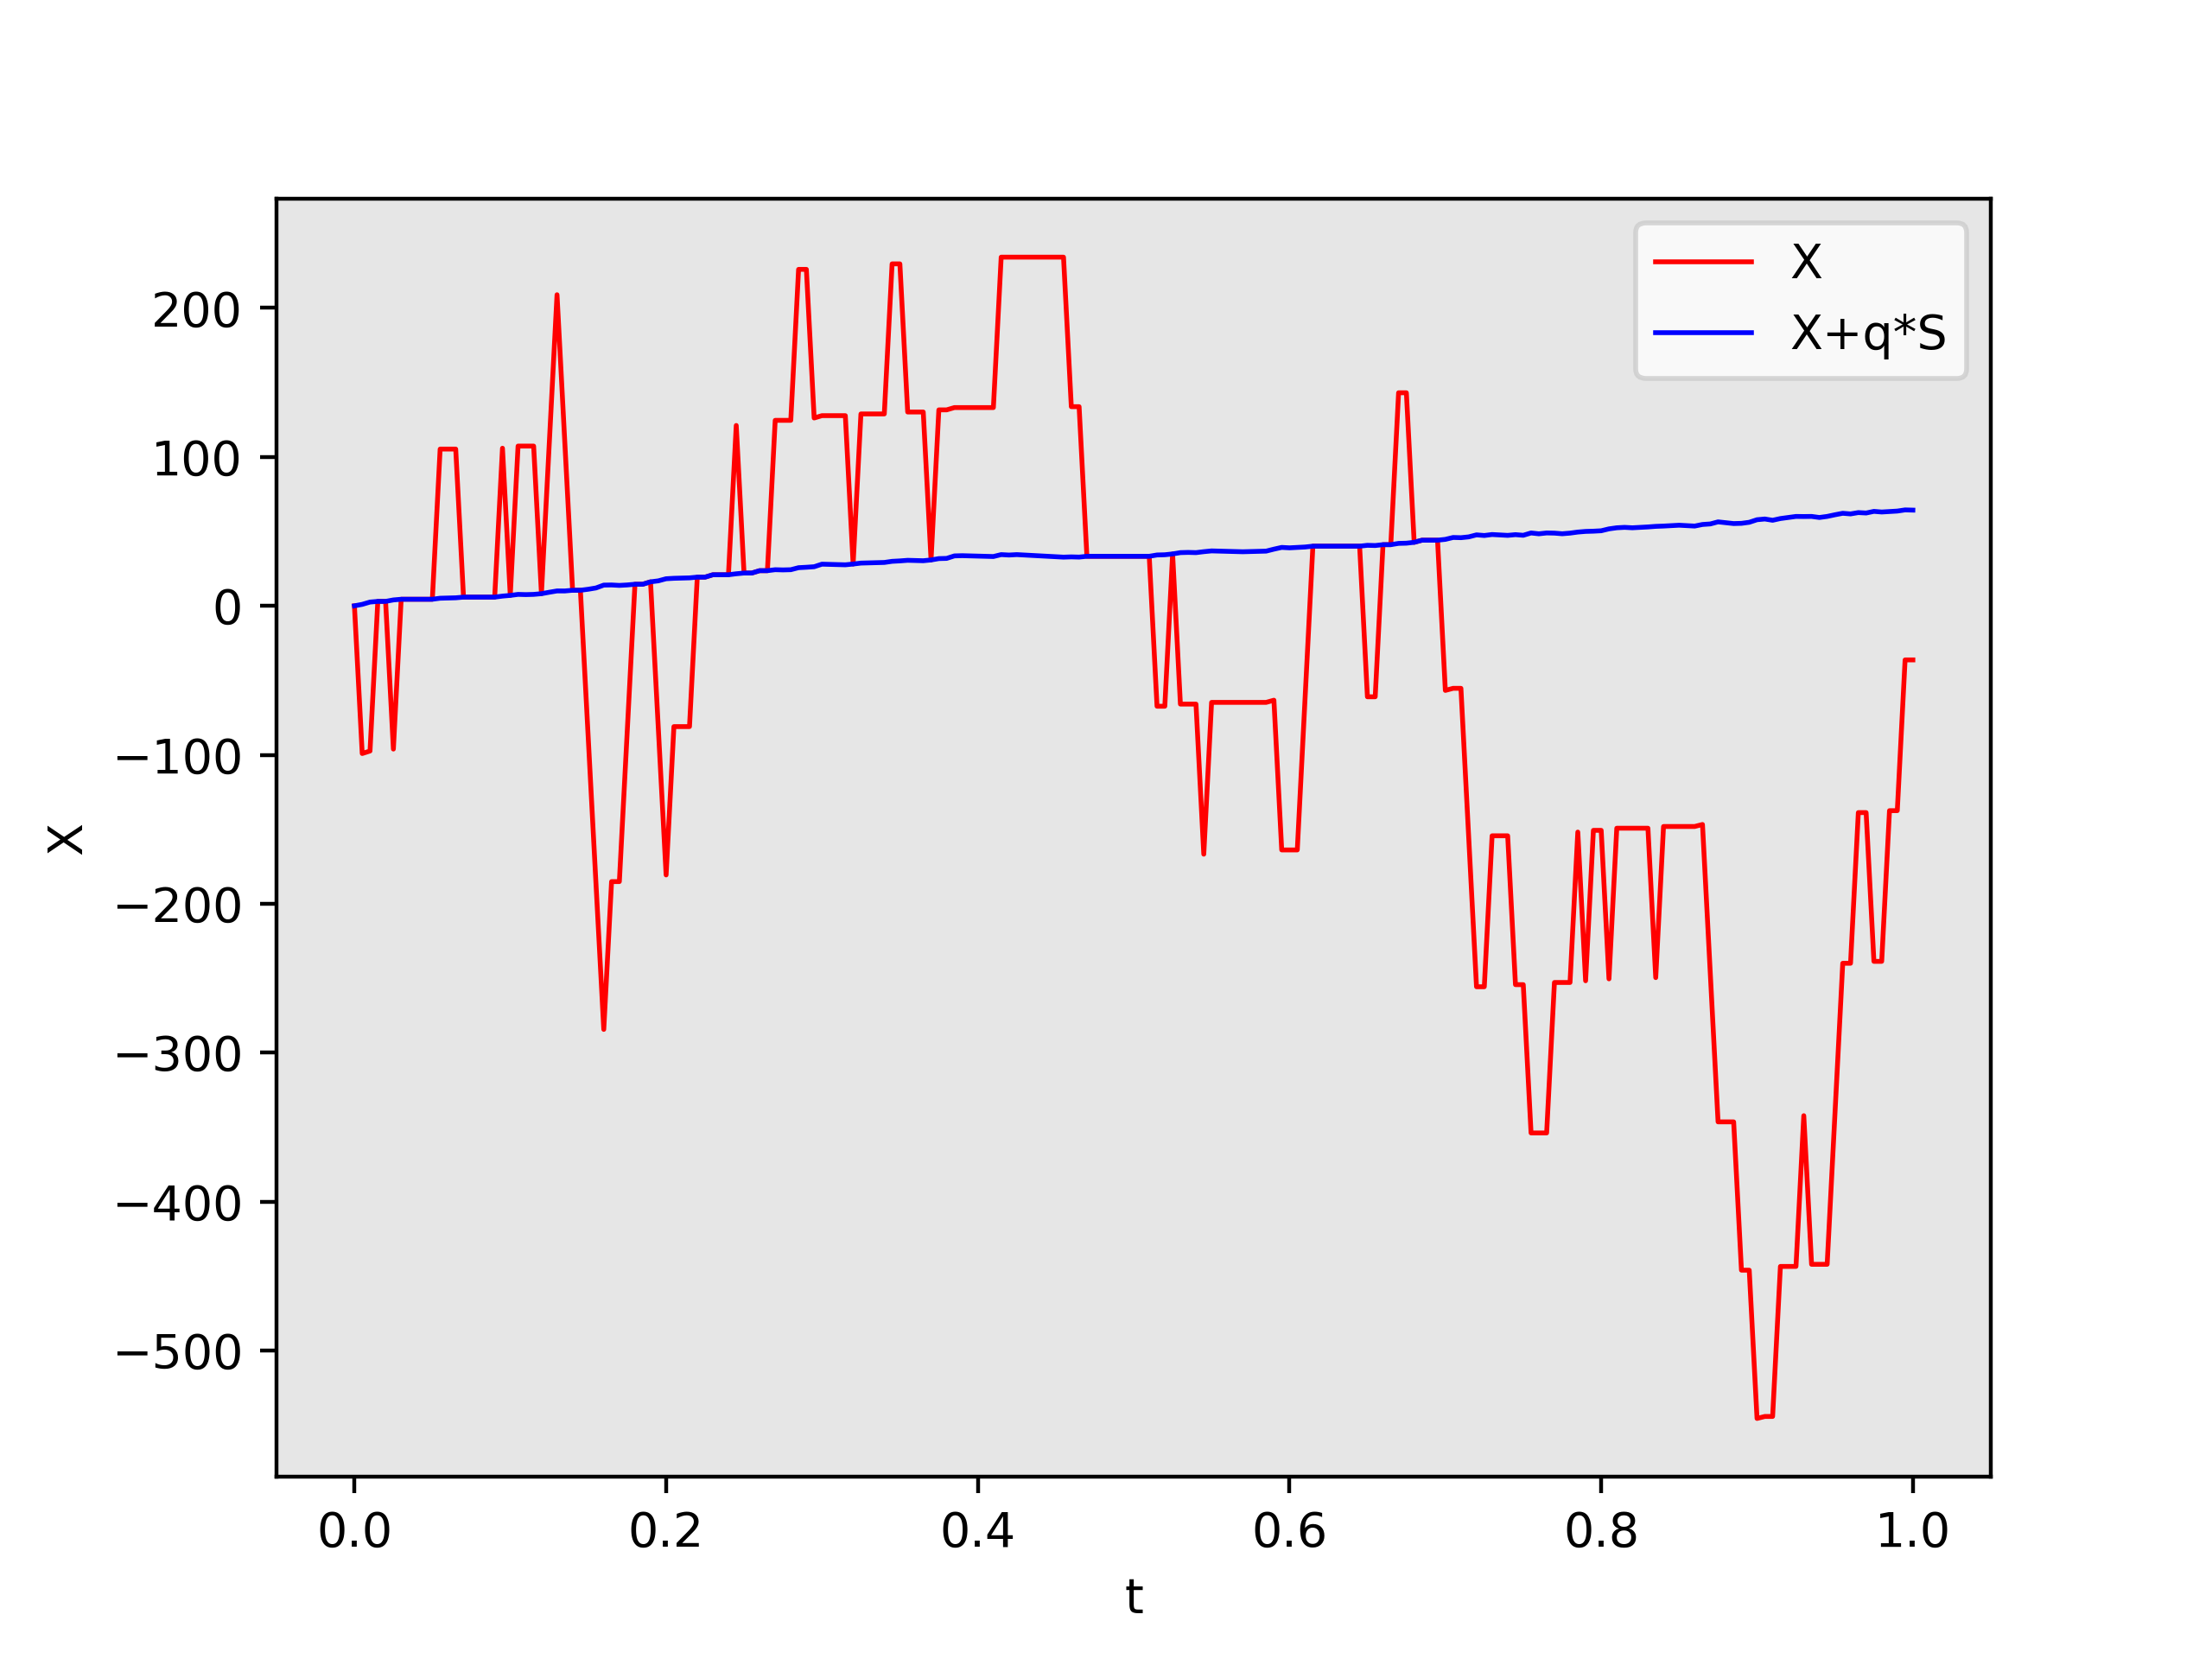
\includegraphics[scale=0.5]{wealth.png}
        \caption{Sample profit for $\gamma=0.1$}
        \label{fig:pnl}
\end{figure}

%\section{Simulation of Extended Model for GBM}
%\section{Estimation of Order Book Parameters for Real-World Data}
%\section{Market Making in the Binance Order Book}